% Figure from MATH 556 notes, section 13. Compile with the notes preamble.
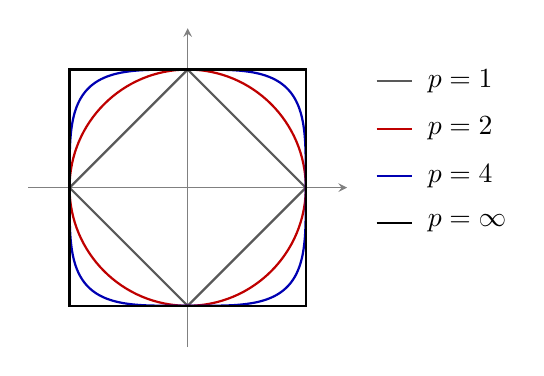
\begin{tikzpicture}[scale=1.5, >=stealth]
    \draw[->, gray] (-1.35,0) -- (1.35,0);
    \draw[->, gray] (0,-1.35) -- (0,1.35);
    \draw[thick, gray!70!black] (1,0) -- (0,1) -- (-1,0) -- (0,-1) -- cycle;
    \draw[thick, red!75!black] (0,0) circle (1);
    \draw[thick, blue!70!black, smooth, domain=0.5:360.5, samples=181]
        plot ({sign(cos(\x))*abs(cos(\x))^(0.5)}, {sign(sin(\x))*abs(sin(\x))^(0.5)});
    \draw[thick] (-1,-1) rectangle (1,1);
    \foreach \y/\st/\lab in {0.9/{gray!70!black}/{$p = 1$}, 0.5/{red!75!black}/{$p = 2$}, 0.1/{blue!70!black}/{$p = 4$}, -0.3/{black}/{$p = \infty$}} {
        \draw[thick, \st] (1.6,\y) -- (1.9,\y);
        \node[anchor=west] at (1.95,\y) {\lab};
    }
\end{tikzpicture}
